\begin{figure*}[!htbp]
\centering
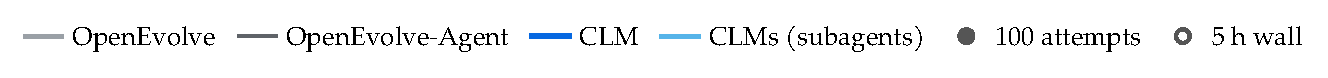
\includegraphics[width=\linewidth]{figures/open_problems/progress_legend.pdf}\\[-6pt]
\begin{subfigure}[t]{0.255\linewidth}\centering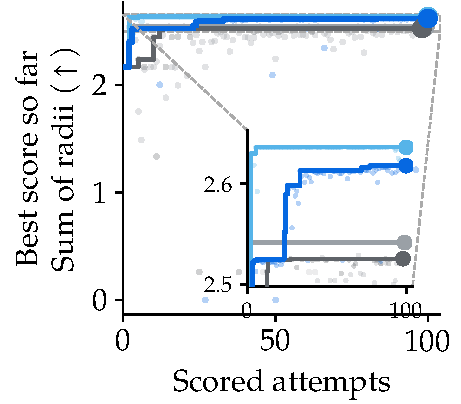
\includegraphics[width=\linewidth]{figures/open_problems/progress_a.pdf}\caption{Circle packing ($\uparrow$).}\label{fig:openended_a}\end{subfigure}\hfill
\begin{subfigure}[t]{0.245\linewidth}\centering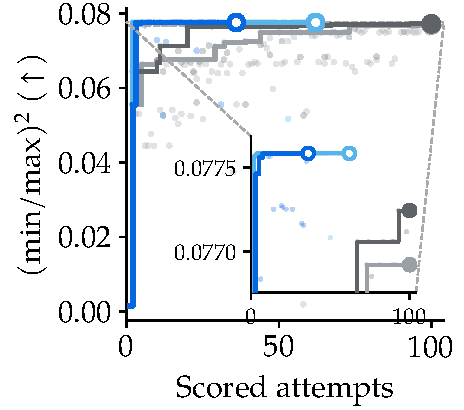
\includegraphics[width=\linewidth]{figures/open_problems/progress_b.pdf}\caption{Min-max/min-dist ($\uparrow$).}\label{fig:openended_b}\end{subfigure}\hfill
\begin{subfigure}[t]{0.245\linewidth}\centering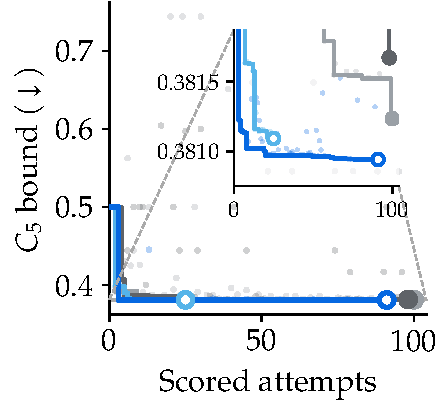
\includegraphics[width=\linewidth]{figures/open_problems/progress_c.pdf}\caption{Erd\H{o}s min-overlap ($\downarrow$).}\label{fig:openended_c}\end{subfigure}\hfill
\begin{subfigure}[t]{0.245\linewidth}\centering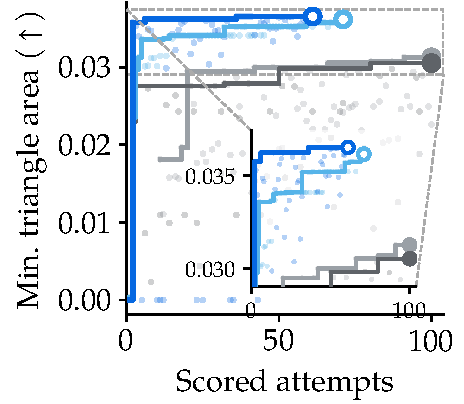
\includegraphics[width=\linewidth]{figures/open_problems/progress_d.pdf}\caption{Heilbronn triangle ($\uparrow$).}\label{fig:openended_d}\end{subfigure}
\caption{\textbf{Best-so-far score versus evaluator-scored attempts on four open optimization problems.}
All runs use Claude 4.6 Sonnet with a 32K context limit and stop after 100 attempts or five hours. Lines show the best score so far, dots individual scored candidates, and insets the final-score range.}
\label{fig:openended-progress}
\end{figure*}
